%!TEX root = p2p-private-cloud.tex

\NewScheme{\SPOR}{SPOR}

\subsection{\Acf*{SPOR}}%
\label{SPOR}%
\label{sec:SPOR}%
\label{sec:message_passing}%

\commentAL{I would like to merge that with \ref{ssec:por}.}

Say that Alice wants to send a message \(m\) to Bob.
Bob creates a reply header using \(\CreateReply\) and gives the output to Alice 
over an out-of-band channel.
%We assume that \(m\) is either unavailable when the channel is used or too large to be successfully sent over the channel directly.
At a later point, Alice attaches a message \(m\) to the reply header using 
\(\UseReply\), creates a forward header using \(\CreateFwd\) with the prepared 
reply header as parameter.
\commentAL{Unclear: she sends? Then it reaches Alice?} Then she sends this packet to the first node, which processes it using 
\(\ProcessHeader\).
The node will then process the header and in turn forward the packet to the 
next node.
At some point the message will reach Alice who identifies the message as the 
one expected to come from Bob.
(This process is illustrated in \cref{fig:file-transfer}.)
Now we will focus on how Alice and Bob choose the nodes that they provide to 
\(\CreateReply\) and \(\CreateFwd\).

\begin{figure}
  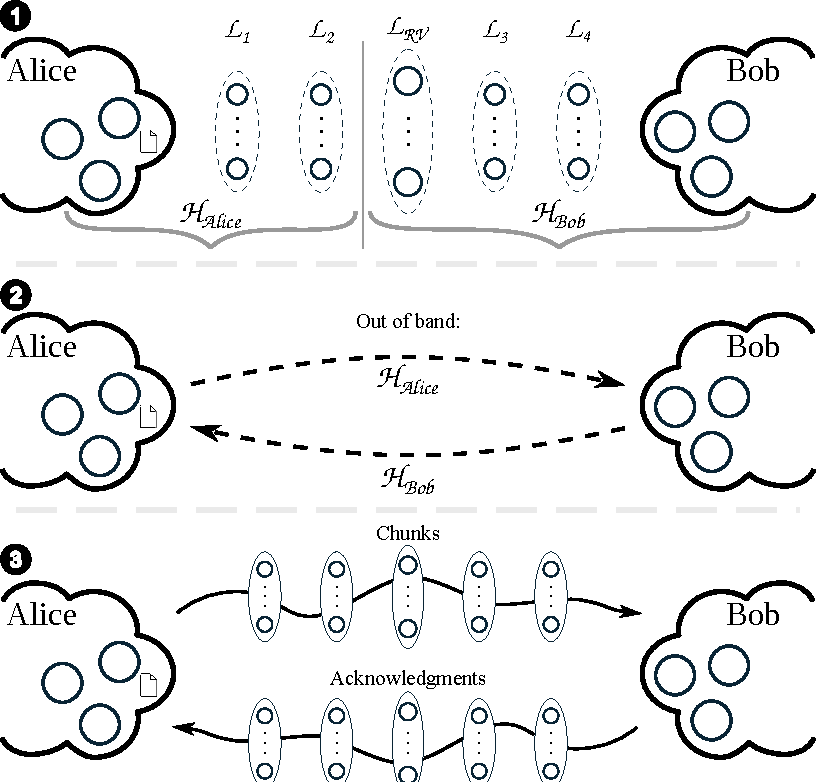
\includegraphics[width=\linewidth]{figures/file_transfer_v2.pdf}
  \caption{\label{fig:file-transfer}%
    A schematic of Alice and Bob sending a message using \name.
    \ding{182} illustrates the layer of the headers that Alice and Bob create.
    In \ding{183}, Alice and Bob exchange the headers out-of-band.
    In \ding{184}, Alice and Bob use two \ac{SPOR} routes, one for messages and 
    one for acknowledgements.
    \commentDaniel{We must update the notation in this figure.}
  }
\end{figure}

\commentAL{When is CreateHeader used?}

There are many uses of Sphinxes, many criteria that can be used to select the 
nodes in each layer.
We will focus on maximizing availability when routing in a network with high 
churn, but one could equally well select nodes to maximize, \eg, bandwidth.
We now describe a protocol, \ac{SPOR}, which uses Sphinxes to transfer messages 
from a source to a destination over a network of nodes with high churn.

\((d, \pk_d, \avail_d)\gets \GetRandomNode\): We assume that there is an 
algorithm \(\GetRandomNode\) which returns a tuple \((d, \pk_d, \avail_d)\) of 
one uniformly randomly selected node, where.
\begin{itemize}
  \item \(d\) is the node's identifier (address);
  \item \(\pk_d\) is the node's public key;
  \item \(\avail_d(t)\) is the node's probability of being online as a function 
    of time.
\end{itemize}
The \(\GetRandomNode\) algorithm can be instantiated using \eg
Octopus~\cite{Octopus}.
But even a solution like Tor's authoritative directory servers would work,
We will treat \(\avail_d\) in \cref{sec:squad_overlay}.

When Bob runs \(\CreateReply\) (or Alice runs \(\CreateFwd\)) he must supply a 
set of nodes for each layer of the route, \(L = \{L_0, \dotsc, L_\nu\}\), where 
\(|L_i| \leq w_L\) for \(0\leq i\leq \nu\).
The set \(L_\nu\) contains only one or more of Bob's devices.
For the other layers, \(L_i\) for \(i < \nu\), Bob will do the following:
Bob queries \(\GetRandomNode\) \((\nu-1)\cdot w_L\) times to get enough nodes 
to fill all remaining layers.
Bob will distribute these nodes across all layers \(L_i\) to maximize \(\min_i 
  \avail_{L_i}(t)\), where \(\avail_{L_i}(t) = 1-\prod_{l\in L_i} 
  (1-\avail_l(t))\).
This means that Bob minimizes the risk of a layer (\ie all nodes in a layer) 
being unavailable.

